\documentclass{minimal}

\usepackage{graphicx}
\usepackage{tikz}
\usetikzlibrary{positioning}
\usetikzlibrary{shapes.geometric}

\begin{document}

\begin{tikzpicture}[
networknode/.style={regular polygon,regular polygon sides=4, draw=black, fill=none, very thick, inner sep=-5pt},
vectornode/.style={rectangle, draw=black, fill=none, very thick, minimum size=5mm},
imagenode/.style={rectangle, draw=none, fill=none, very thick, minimum size=5mm},
]
%Nodes
% What sorta style should the text have? Blue ass well?
% mention a cnn somewhere
% also see https://www.researchgate.net/figure/The-high-level-concept-of-an-extended-variational-autoencoder-adopted-for_fig8_317486066
\node[networknode] (encoder) {\textbf{Encoder Network}\\\newline(5CNN)};
\node[vectornode] (latent) [right=of encoder] {$\sum^2{x+1}$};
\node[networknode] (decoder) [right=of latent] {\textbf{Decoder Network}};
\node[imagenode] (output) [right=of decoder] {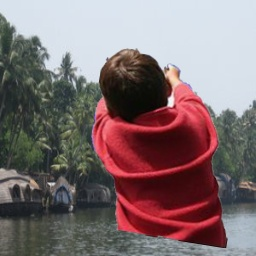
\includegraphics[width=0.2\textwidth]{syn1}};

%Lines
\draw[->] (encoder.east) -- (latent.west);
\draw[->] (latent.east) -- (decoder.west);
\draw[->] (decoder.east) -- (output.west);
%% \draw[->] (decoder.west) .. controls +(down:7mm) and +(right:7mm) .. (lowercircle.east);
%% \draw[->] (decoder.west) 

\end{tikzpicture}

\end{document}
